\section{Experimentación - PageRank y páginas web}
	A continuación, se presentan los experimentos que se realizaron. Con el código del trabajo práctico se incluye una serie de scripts de \emph{bash} que permiten recrear los experimentos realizados, como así también los gráficos que se incluyen en este informe; esto puede hacerse ingresando al directorio \texttt{exp} dentro de la raíz, y ejecutando el comando \texttt{./expi.sh} siendo i el número de experimento.

	\subsection{Experimento 1}
	En el primer experimento se quiere observar como varía el tiempo de ejecución a medida que se modifica el valor del parámetro c, para lograr que la norma Manhattan entre dos iteraciones consecutivas sea menor que la tolerancia indicada. Para ello se toma una determinada cantidad de páginas web que no se modificarán a lo largo del experimento y se ejecutará el programa para diferentes valores de c. 

		\subsubsection*{Hipótesis} 
		Se conjetura que cuanta mayor sea la probabilidad de teletransportarse de una página a otra, menos tiempo va a tardar el algoritmo en llegar al estado en el que la tolerancia sea menor que la norma Manhattan. (1-c) indica cual es la probabilidad de estando en cualquier página teletransportarse a otra. Por esto es que cuanto más chico sea el valor de c, menos tiempo de ejecución demorará el algoritmo.

		\subsubsection*{Valores utilizados como parámetros} 
		Se toman 13 páginas con 16 links. Además el parámetro c toma los valores 0 0.1 0.2 0.3 0.4 0.5 0.6 0.7 0.8 0.9 1. La tolerancia es de 0.00001.

		\subsubsection*{Resultados}
			{\centering \begin{tabular}{c}
		      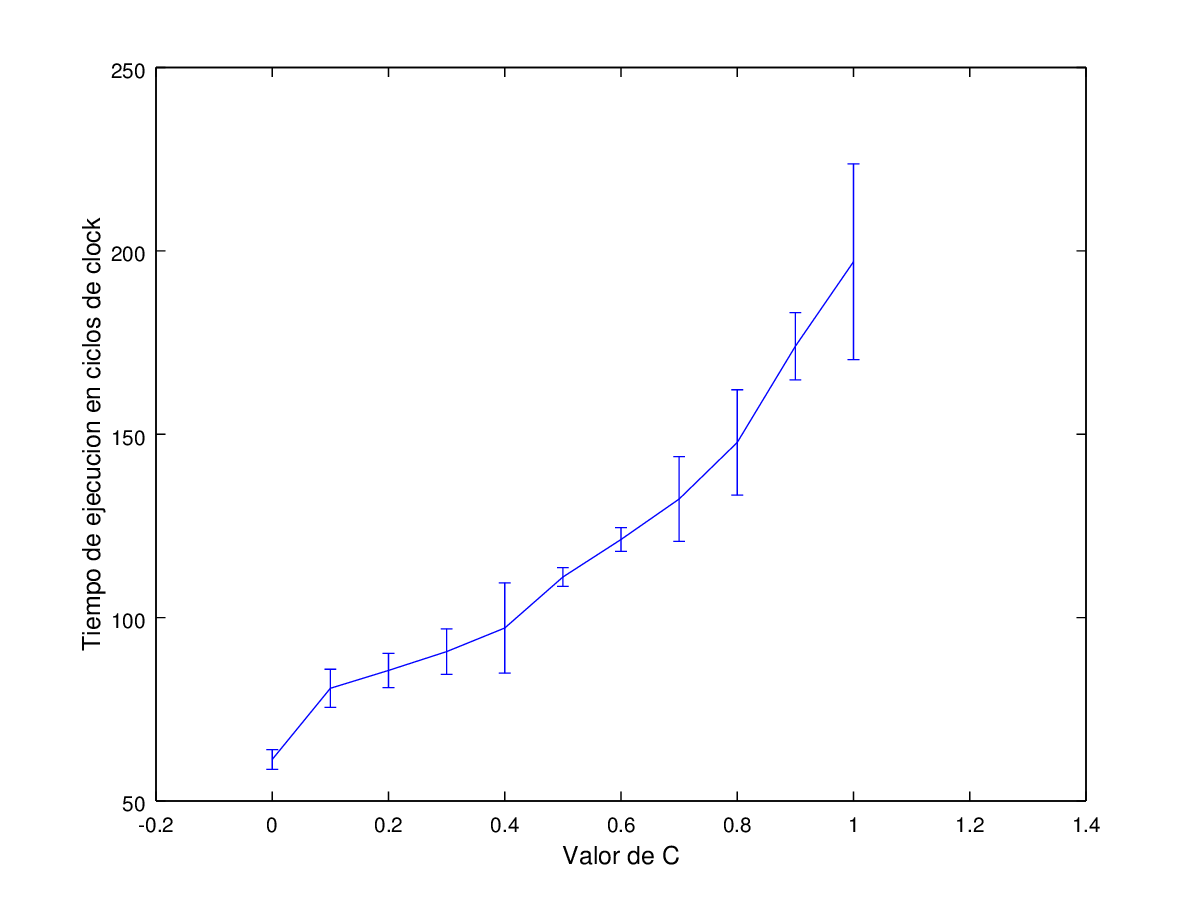
\includegraphics[width=12cm]{../../src/exp/graficos/exp1.png} \\
		    \end{tabular}}

		\subsubsection*{Conclusiones y observaciones} 
		Como se puede observar en el experimento, a medida que aumenta el valor de c, aumenta el tiempo de ejecución. Esto se debe a que la matriz inicial no es homogénea y la que formamos a partir del c si lo es. Así, cuando la segunda toma dicha importancia, el sistema tiende más rápido a ser homogéneo y requiere menos iteraciones del ciclo para lograr una norma menor a la tolerancia deseada. 



	\subsection{Experimento 2}
	El objetivo de este experimento se pretende observar la diferencia en el tiempo de ejecución cuando se varía la cantidad de links en una determinada cantidad de páginas manteniendo el valor de la tolerancia constante.

	Para ello se utilizan listas de páginas diferentes como parámetro de entrada en cada una de las ejecuciones a comparar, pero manteniendo la cantidad de las mismas. Se toma el tiempo que se demora en ejecutar el algoritmo y se lo divide por la cantidad de iteraciones realizadas. Esto permite obtener un promedio del tiempo que demora por cada una de las iteraciones del ciclo. 
	


		\subsubsection*{Hipótesis} 
			Suponemos que variar la cantidad de links altera más el tiempo de ejecución que variar la cantidad de páginas sin que estén relacionadas entre ellas. Esto se debe a que en la implementación para las páginas que no están relacionadas solamente se realiza un cáculo sencillo a diferencia de las que si lo están. Por lo tanto, se espera observar que el tiempo de ejecución aumente a medida que la cantidad de relaciones entre páginas sea mayor. 

		\subsubsection*{Valores utilizados como parámetros} 		
		Para este experimento se toman 50 páginas. La cantidad de links entre ellas varía, tomando los valores 4 32 70 105 130 160. Además el valor de c es 0.85 y el valor de la tolerancia es 0.00001. 
		
		\subsubsection*{Resultados}
			{\centering \begin{tabular}{c}
		      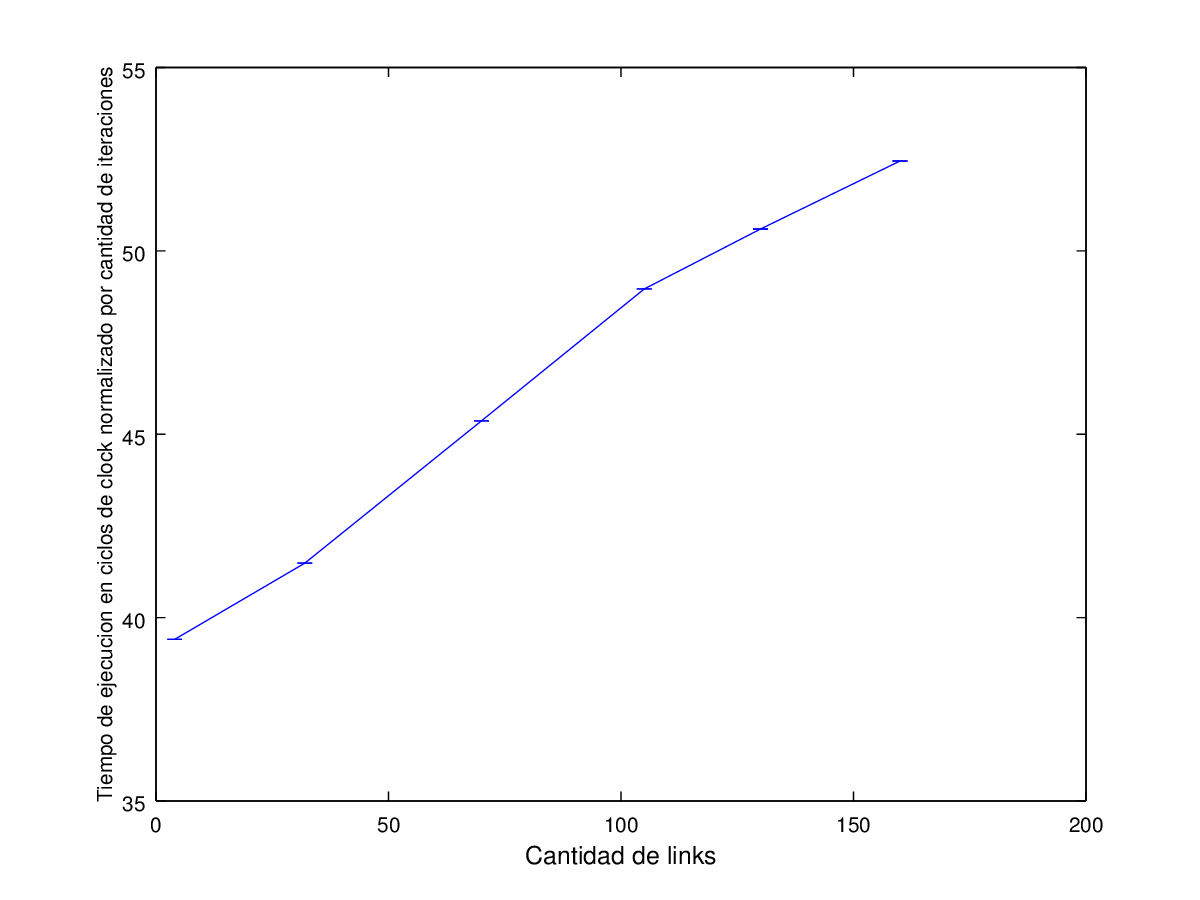
\includegraphics[width=12cm]{../../src/exp/graficos/exp2.png} \\
		    \end{tabular}}


		\subsubsection*{Conclusiones y observaciones}
		Como se puede observar en el gráfico, a medida que aumentan las relaciones entre las páginas el tiempo de ejecución es mayor.  



	\subsection{Experimento 3}
	En este experimento también se observa la diferencia en el tiempo de ejecución pero comparando igual cantidad de páginas y relaciones entre las mismas y variando el valor de la tolerancia.

	Para ello se toma como parámetro de entrada en cada una de las ejecuciones una misma lista de páginas y se incrementa el valor de la tolerancia.

		\subsubsection*{Hipótesis} 
		Creemos que cuanto mayor sea la tolerancia, menor será el tiempo de ejecución del algoritmo. Esto se debe a que el algoritmo termina cuando la diferencia Manhattan es menor que la tolerancia. Entonces cuanto más grande sea el valor de la tolerancia, más rápido se cumplirá la condición para salir del ciclo y menos tardará en ejecutarse el algoritmo. 

		\subsubsection*{Valores utilizados como parámetros} 
		Se toman 13 páginas con 16 links. Además la tolerancia toma los valores 0.000001 0.000005 0.00001 0.00005 0.0001 0.0005 0.001 0.005 0.01 0.1 0.3 0.5 0.7. El parámetro c es igual a 0.85.

		\subsubsection*{Resultados}
			{\centering \begin{tabular}{c}
		      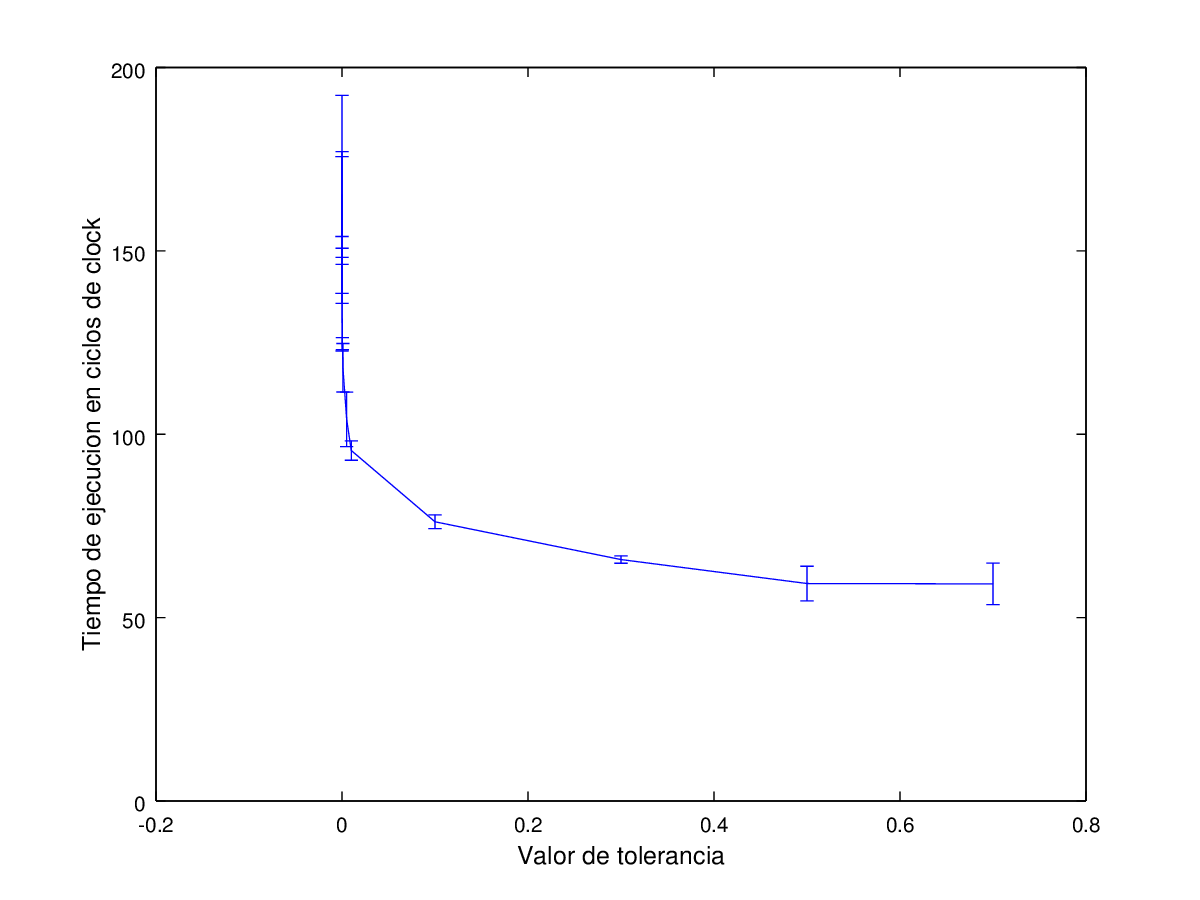
\includegraphics[width=12cm]{../../src/exp/graficos/exp3.png} \\
		    \end{tabular}}

		\subsubsection*{Conclusiones y observaciones}
		Como se puede ver en el gráfico, al aumentar la tolerancia disminuye el tiempo de ejecución. En este sentido, se pudo confirmar la hipótesis.  

	

	\subsection{Experimento 4}
	Otra de las pruebas consiste en comparar los rankings formados al ejecutar los algoritmos de PageRank y el de INDEG. Primero se analiza una lista de páginas de entrada en la que una de ellas sea apuntada por el resto (Web 1). 

	Luego se realiza la comparación con una lista en la que hayan dos páginas (a las que llamaremos página 1 y página 3) que sean apuntadas por varias paginas. Además, la página 3 tendrá un link a la 1. También se cuenta con otra (a la que llamaremos página 2) que apunta y es apuntada por la página 1, tal como se muestra en el siguiente esquema (Web 2):

			{\centering \begin{tabular}{c}
		      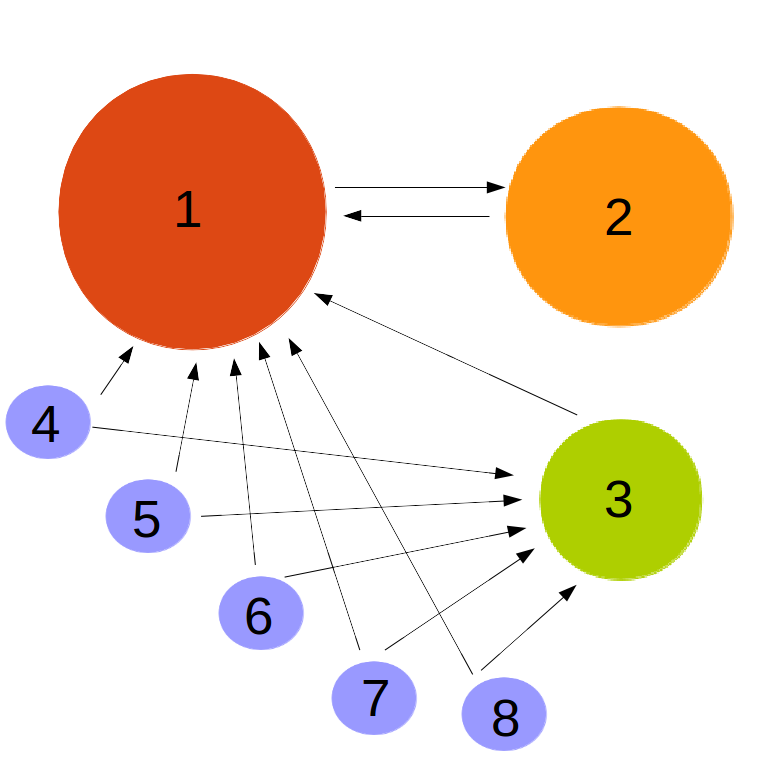
\includegraphics[width=6cm]{../../src/exp/graficos/exp4-graph.png} \\
		    \end{tabular}}

		\subsubsection*{Hipótesis} 
		En el primero, suponemos que los rankings obtenidos en ambos casos serán iguales ya que existe una sola página principal y el resto tiene igual cantidad de relaciones. Por otro lado, en el segundo notaremos diferencias. Llamaremos enlace fuerte a aquel que va de una página que es apuntada por muchas otras hacia otra página. El método PageRank tiene en cuenta cual es el peso de los links que apuntan a las distintas páginas. En el caso de INDEG solo se utiliza como información la cantidad de enlaces que llegan a cada una de las distintas páginas.

		En el experimento, si consideramos el método PageRank, la página 1 quedará en primer lugar ya que es la que recibe más links a la misma, pero en segundo lugar quedará la página 2. Esto se debe a que el enlace de la 1 a la 2 es un enlace muy fuerte. En el caso de INDEG, esto no sucede ya que este método solo toma en cuenta que existe un único link hacia la página 2. Por lo tanto en PageRank las posiciones serán 1-2-3 y luego el resto. En INDEG tendremos primero a la página 1 seguida de la 3, luego la 2 y finalmente el resto.

		\subsubsection*{Valores utilizados como parámetros}
		 		

		\subsubsection*{Resultados}


		   \begin{center}
      			\begin{tabular}{c|c|c} 
		      		\hline
		  				\multicolumn{3}{c}{Ranking Web 1 - PageRank} \\
		 			\hline
        			Posición & Nodo & Puntaje \\ \hline
         			1 & 1 & 0.473848 \\
        			2 & 8 & 0.078821 \\
        			3 & 9 & 0.078821 \\
        			4 & 2 & 0.061418 \\
        			5 & 3 & 0.061418 \\
        			6 & 4 & 0.061418 \\
        			7 & 5 & 0.061418 \\
        			8 & 6 & 0.061418 \\
        			9 & 7 & 0.061418 
      			\end{tabular} 

      			\begin{tabular}{c|c|c}
		      		\hline
		  				\multicolumn{3}{c}{Ranking Web 1 - INDEG} \\
		 			\hline
        			Posición & Nodo & Puntaje \\ \hline
         			1 & 1 & 0.8 \\
        			2 & 8 & 0.1 \\
        			3 & 9 & 0.1 \\
        			4 & 2 & 0 \\
        			5 & 3 & 0 \\
        			6 & 4 & 0 \\
        			7 & 5 & 0 \\
        			8 & 6 & 0 \\
        			9 & 7 & 0 
      			\end{tabular}

      			\begin{tabular}{c|c|c}
		      		\hline
		  				\multicolumn{3}{c}{Ranking Web 2 - PageRank} \\
		 			\hline
        			Posición & Nodo & Puntaje \\ \hline
         			1 & 1 & 0.448059 \\
        			2 & 2 & 0.448059 \\
        			3 & 3 & 0.058594 \\
        			4 & 4 & 0.058594 \\
        			5 & 5 & 0.018750 \\
        			6 & 6 & 0.018750 \\
        			7 & 7 & 0.018750 \\
        			8 & 8 & 0.018750
      			\end{tabular}
    		
      			\begin{tabular}{c|c|c}
		      		\hline
		  				\multicolumn{3}{c}{Ranking Web 2 - INDEG} \\
		 			\hline
        			Posición & Nodo & Puntaje \\ \hline
         			1 & 1 & 0.538462 \\
        			2 & 3 & 0.384615 \\
        			3 & 2 & 0.076923 \\
        			4 & 4 & 0 \\
        			5 & 5 & 0 \\
        			6 & 6 & 0 \\
        			7 & 7 & 0 \\
        			8 & 8 & 0 \\
      			\end{tabular}
    	\end{center}

		\subsubsection*{Conclusiones y observaciones} 
		Como podemos ver en los rankings del primer análisis en ambos casos quedan iguales. En cambio en el segundo observamos variaciones ya que en la lista de entrada el peso de todos los enlaces no es el mismo, es decir, hay enlaces más fuertes que otros. A diferencia de PageRank, el método INDEG no tiene en cuenta esta propiedad. Por lo tanto, si en las páginas de entrada todos los links tienen igual fuerza, el resultado obtenido por ambos métodos no difiere. 

\section{Experimentación - PageRank y ligas deportivas}
	

	\subsection{Experimento 1}
	En este experimento se verá la diferencia entre los métodos de pageRank y el de la AFA para determinar el ranking de una liga deportiva. Para ello se tomará como parámetro de entrada una tabla con los partidos, sus respectivas fechas, y sus resultados. En la misma, deberá existir un equipo que ocupe una de las primaras posiciones en la tabla de rankings que haya perdido contra otro que ocupa una de las últimas. Observaremos la diferencia entre el ranking generado por cada uno de los métodos.
		

		\subsubsection*{Hipótesis} 
		Cuando se juega un partido entre dos equipos, en el método de pageRank se tendrá en cuanta que tan fuerte son los equipos involucrados y cual fue la diferencia de goles en el partido. En cambio, en el método de la AFA el ganador recibirá 3 puntos sin importar los resultados ni las posiciones que los mismos tenían hasta el momento. Esto puede generar diferencias en el ranking ya que cada método considera distinta información para determinar las nuevas posiciones. 
		
		Por otro lado, si un equipo malo juega contra uno bueno y gana el peor, para el método de la AFA es exactamente igual que que haya jugado con cualquier otro. Para pageRank, al tener en cuenta que tan fuertes son los equipos, esto generará que el nuevo vencedor quede en una mejor posición en la tabla. Así en este método entre dos fechas se pueden generar saltos, es decir, un equipo puede pasar de tener una muy mala posición en la tabla a estar dentro de los mejores solo por haber ganado un partido contra un equipo fuerte. En el método de la AFA no pasa ya que sólo se le sumarán 3 puntos al equipo triunfador. Si éste se encontraba en las ultimas posiciones de la tabla no podrá ascender más de 3 posiciones. 		

		\subsubsection*{Valores utilizados como parámetros} 

		\subsubsection*{Resultados}

		\subsubsection*{Conclusiones y observaciones} 

	\subsection{Experimento 1}

		\subsubsection*{Hipótesis}
